\documentclass[12pt]{report}

% --------- Encodage & langue ---------
\usepackage[utf8]{inputenc}
\usepackage[T1]{fontenc}
\usepackage[french]{babel}
\usepackage{csquotes}

% --------- Mise en page ---------
\usepackage[a4paper,margin=2.5cm]{geometry}
\usepackage{setspace}
\onehalfspacing{}
\usepackage{lastpage}
\setlength{\parindent}{0pt}
\setlength{\intextsep}{0pt}
\setlength{\columnsep}{20pt}
\usepackage{wrapfig}
\usepackage{multicol}
\usepackage{caption}

% --------- Graphiques et figures ---------
\usepackage{graphicx}
\usepackage[dvipsnames]{xcolor}
\usepackage{subfigure}
\usepackage{float}
\usepackage{floatflt}
\usepackage{makecell}
\usepackage{subcaption}
\usepackage{tikz}
\usepackage{pgfplots}
\pgfplotsset{compat=1.18}

\usetikzlibrary{decorations.pathreplacing, fit, backgrounds, calc, shapes.geometric, arrows.meta, positioning, shadows.blur}

\tikzset{
  box/.style={
    rectangle, rounded corners, minimum width=4cm, minimum height=1.2cm,
    text centered, draw=black, fill=blue!20,
    drop shadow={shadow xshift=0.5ex,shadow yshift=-0.5ex,opacity=0.2}
  },
  service/.style={
    rectangle, rounded corners, minimum width=3.8cm, minimum height=1cm,
    text centered, draw=black, fill=green!25,
    drop shadow={shadow xshift=0.3ex,shadow yshift=-0.3ex,opacity=0.15}
  },
  departement/.style={
    rectangle, rounded corners, minimum width=5cm, minimum height=1.1cm,
    text centered, draw=black, fill=orange!30,
    drop shadow={shadow xshift=0.4ex,shadow yshift=-0.4ex,opacity=0.2}
  },
  conseil/.style={
    rectangle, rounded corners, minimum width=5.2cm, minimum height=1.1cm,
    text centered, draw=black, fill=red!30,
    drop shadow={shadow xshift=0.4ex,shadow yshift=-0.4ex,opacity=0.2}
  },
  arrow/.style={
    ->,>=Stealth, line width=0.4pt, color=gray!60
  }
}

% --------- Code et algorithmes ---------
\usepackage{listings}
\usepackage{algpseudocode}
\usepackage{algorithm}
\lstset{
  basicstyle=\ttfamily\small,
  numbers=left,
  numberstyle=\tiny,
  frame=single,
  breaklines=true
}

% --------- Math, couleurs, liens ---------
\usepackage{amsmath, amssymb}
\usepackage{xcolor}
\usepackage{hyperref}
\hypersetup{
    colorlinks=true,
    linkcolor=blue,
    urlcolor=blue,
    citecolor=blue
}

% --------- Bibliographie ---------
\usepackage[backend=biber,style=ieee]{biblatex}
\addbibresource{bibliographie.bib} % ton fichier .bib

\begin{document}
\pagenumbering{gobble}

% --------- Page de garde ---------
\begin{minipage}{0.5\textwidth}
    
\includegraphics[width=7cm]{logo-prepa.png}
\end{minipage}
\hfill

\vspace{2cm}

\begin{center}
    \Large \textbf{DELAGE Florian} \\
    \vspace{0.5cm}
    \normalsize Année 2024--2025 \\
    Promotion 31 \\
    
    \vspace{1.5cm}
    \large \textbf{Rapport de stage\ --\ Loria} \\
    \textbf{Période : du 05 mai au 13 juin 2025} \\
    
    \vspace{1.5cm}
    \Huge \textbf{Optimisation d'un algorithme de calcul de bornes de latences pour accélérer la génération de preuves} \\
    
    \vspace{1.5cm}
    \normalsize \textit{Encadrants :} \\
    AMET Matthieu\\
    THOMAS Ludovic
    

    \vspace{1cm}
    \normalsize \textit{Coordonnées de l'entreprise :} \\
    Loria, 54506 Vandœuvre-lès-Nancy Cedex\\
    Tél : +33 3 83 59 20 00
\end{center}

\vfill

% Logos en bas
\begin{center}
    \begin{minipage}{\textwidth}
        \centering
        
\includegraphics[width=10cm]{logo-l-inp.png}
    \end{minipage}
\end{center}
\thispagestyle{empty}


% --------- Remerciements ---------
\chapter*{Remerciements}
\vspace{1em}
Je tiens à remercier chaleureusement l'ensemble des personnes qui ont 
contribué au bon déroulement de mon stage au sein du Loria.
Je remercie tout particulièrement monsieur Matthieu AMET, mon maître de 
stage, ainsi que monsieur Ludovic THOMAS pour leur accueil, leur disponibilité, 
leur conseil et l'accompagnement qu'ils m'ont apporté tout au long de cette expérience. 
Leur encadrement m'a permis de progresser aussi bien sur le plan 
professionnel que personnel.
Je souhaite également exprimer ma gratitude à toute l'équipe SIMBIOT, 
pour leur bienveillance, leur écoute et leur esprit collaboratif, 
qui ont largement facilité mon intégration.
Enfin, je remercie monsieur Théo DOCQUIER pour son suivi et son soutien 
dans la réalisation de ce stage.

% --------- Résumé ---------
\chapter*{Résumé}
\vspace{1em}

Au cours de mon stage au sein de l'équipe SIMBIOT du laboratoire Loria 
(Université de Lorraine), j'ai travaillé sur l'optimisation d'un algorithme 
de calcul de bornes de latence (Total Flow Analysis\ --\ TFA) dans le 
contexte des réseaux temps-réels. L'objectif était d'accélérer la 
génération de preuves à divulgation nulle de connaissance (Zero-Knowledge Proofs) à l'aide de l'outil Risc Zero, 
sans compromettre l'exactitude des résultats.

\vspace{0.2cm}

Mes contributions principales ont été les suivantes :
\begin{itemize}
    \item Analyse des performances de l'algorithme TFA existant, en identifiant les goulots d'étranglement dans l'algorithme ;
    \item Optimisation du code en Rust, pour maximiser l'efficacité des calculs ;
    \item Exploration et intégration de techniques de réduction des coûts cryptographiques, afin d'accélérer la génération des ZKP (Zero-Knowledge Proofs) tout en respectant les contraintes liées à la génération de preuves de Risc Zero.
\end{itemize}

\vspace{0.2cm}

J'ai pu également aider à l'implémentation d'une extension moins pessimiste de TFA (TFA++)
Ce projet s'inscrit dans une démarche d'innovation visant à rendre 
les applications critiques utilisant des réseaux temps-réels viables à
grande échelle.


\tableofcontents
\newpage

% --------- Introduction ---------
\chapter{Introduction}
\pagenumbering{arabic}
\setcounter{page}{1}

À mesure que la technologie progresse, de plus en plus de systèmes 
reposent sur des échanges d'informations rapides, fiables et 
prévisibles. C'est notamment le cas des voitures autonomes,
des satellites, ou encore des chaînes de 
production automatisées. Dans ces environnements, il est essentiel que 
les données circulent dans des 
délais garantis. Un simple retard de quelques millisecondes peut entraîner 
des dysfonctionnements majeurs, voire des situations dangereuses. 
C'est pour répondre à ces besoins qu'ont été développés les réseaux 
temps-réels qui visent à offrir des garanties strictes sur la latence 
maximale des communications.\\

Contrairement aux réseaux classiques de type Internet,
les réseaux temps-réels doivent fournir des garanties de latence dans le pire cas. Pour cela, des algorithmes comme Total Flow Analysis 
(TFA) ont été conçus afin d'en calculr des bornes de latence. Ces dernières seront utilisées 
afin de valider le respect des contraintes.\\

Cependant dans des environnements collaboratifs, une nouvelle problématique 
se pose : comment prouver à l'un que les contraintes de latence sont 
respectées par l'autre, sans pour autant lui révéler sa configuration interne ? 
C'est ici qu'intervient une approche innovante issue de la cryptographie : les Zero-Knowledge Proofs 
(ZKP). Ces preuves permettent de démontrer qu'un calcul est correct, 
sans pour autant exposer les données utilisées pour l'effectuer.\\

L'objectif principal de ce stage est d'optimiser un algorithme de calcul de latence 
afin d'accélérer la génération de ZKP. Ceci reste aujourd'hui 
très coûteux en temps et en ressources. Il s'agit donc d'identifier les 
points les plus lents de l'algorithme, et d'explorer des techniques pour rendre le
processus plus rapide.\\

Ce travail s'inscrit dans une perspective plus large : rendre les 
réseaux temps-réels vérifiables, transparents et fiables à grande échelle, 
ce qui pourrait faciliter leur adoption dans des domaines industriels ou 
critiques, où la confiance entre acteurs est primordiale.

% --------- Présentation de l'environnement ---------
\section*{Présentation du laboratoire}

\begin{wrapfigure}{r}{0.3\textwidth}
    \vspace{-10pt}
    
\includegraphics[width=0.28\textwidth]{logo_loria.png}
    \vspace{-10pt}
\end{wrapfigure}

Le Loria, \textbf{Laboratoire lorrain de Recherche en Informatique et 
ses Applications} est une Unité Mixte de Recherche, commune à plusieurs 
établissements : le CNRS, l'Université de Lorraine, CentraleSupélec et 
Inria.

Leurs travaux scientifiques sont divisés en thématiques de recherche à travers 
500 personnes au sein de 5 départements.

\medskip

Ci-dessous un organigramme reprenant l'organisation du laboratoire:

\vspace{1cm}  

\begin{tikzpicture}[font=\sffamily, scale=0.65, transform shape]

% Direction
\node[align=center] (direction) [box] {\textbf{Direction}\\  \small Yannick Toussaint (Directeur) \\ Armelle Brun \& Sylvain Lazard (Directeurs adjoints)};

% Conseils (alignés horizontalement)
\node (conseil_scientifique) [conseil, below=1cm of direction, xshift=1] {Conseil Scientifique};
\node (conseil_labo) [conseil, left=2cm of conseil_scientifique] {Conseil de Laboratoire};
\node (areq) [conseil, right=2cm of conseil_scientifique] {AREQ \\ (Assemblée des Responsables d'Équipes)};

% Départements (alignés verticalement sous conseil_labo)
\node[align=center] (dep1) [departement, below=1cm of conseil_labo, xshift=2cm] {
  \textbf{Département 1} \\
  Algorithmique, calcul, image et géométrie
};
\node[align=center] (dep2) [departement, below=0.5cm of dep1, xshift=-3cm] {
  \textbf{Département 2} \\
  Méthodes formelles
};
\node[align=center] (dep3) [departement, below=0.5cm of dep2] {
  \textbf{Département 3} \\
  Réseaux, systèmes et services
};
\node[align=center] (dep4) [departement, right=0.5cm of dep2] {
  \textbf{Département 4} \\
  Traitement automatique des langues\\ et des connaissances
};
\node[align=center] (dep5) [departement, below=0.5cm of dep4] {
  \textbf{Département 5} \\
  Systèmes complexes, \\intelligence artificielle et robotique
};

% Services (alignés verticalement à droite des départements)
\node (service_gestion) [service, right=7cm of dep1] {Service de Gestion};
\node (service_info) [service, below=0.5cm of service_gestion] {Service Informatique de Soutien à la Recherche};
\node (service_comm) [service, below=0.5cm of service_info] {Service Communication};
\node (transfert) [service, below=0.5cm of service_comm] {Transfert Technologique};

% Flèches direction vers conseils
\draw [arrow] (direction) -- (conseil_scientifique);
\draw [arrow] (direction) -- (conseil_labo);
\draw [arrow] (direction) -- (areq);

% Flèches conseils vers départements
\foreach \dep in {dep1, dep2, dep3, dep4, dep5} {
  \draw [arrow] (conseil_labo) -- (\dep);
}

% Flèches direction vers services, avec courbes plus douces
\draw [arrow] (direction.east) .. controls +(.8,0) and +(-.8,0) .. (service_gestion.west);
\draw [arrow] (direction.east) ++(0,-0.4) .. controls +(.8,0) and +(-.8,0) .. (service_info.west);
\draw [arrow] (direction.east) ++(0,-0.8) .. controls +(.8,0) and +(-.8,0) .. (service_comm.west);
\draw [arrow] (direction.east) ++(0,-1.2) .. controls +(.8,0) and +(-.8,0) .. (transfert.west);

\end{tikzpicture}

\vspace{1cm}

\begin{wrapfigure}{r}{0.23\textwidth}
    \vspace{-3pt}
    
\includegraphics[width=0.20\textwidth]{logo_simbiot.png}
    \vspace{-3pt}
\end{wrapfigure}

Au cours de mon stage, j'ai rejoint l'équipe SIMBIOT, dont la mission est la conception et la validation de systèmes cyber-physiques dits « intelligents ». 
Les travaux de l'équipe se concentrent principalement sur les propriétés d'adaptabilité de ces systèmes, tant au niveau du calcul que des communications, dans le but de renforcer leur autonomie.


% --------- Sujet de stage ---------
\chapter{Sujet du stage}

Dans cette partie, nous allons étudier les différents éléments clés permettant
le calcul des bornes de latences ainsi que la génération de preuves de ces bornes
en questions.

\section*{Calcul des bornes de latences}

L'un des premiers défis de mon stage a été l'étude et la compréhension de l'algorithme 
\textbf{Total Flow Analysis (TFA)}. Il s'agit d'un algorithme d'analyse déterministe
(affirmant, avec certitude, qu'on ne peut dépasser une certaine valeur) utilisé pour estimer des \textbf{bornes de latence dans le pire des cas}. Ces réseaux sont couramment rencontrés dans des environnements critiques où il est nécessaire de garantir le respect de délais stricts, comme dans les systèmes embarqués, les réseaux industriels ou les communications critiques.

\paragraph{Objectif.} L'algorithme TFA sert à estimer, pour chaque flux de données dans un réseau, le temps maximum qu'un message peut mettre pour arriver à destination, en tenant compte de la manière dont le réseau est organisé. Il est conçu pour des systèmes où certains messages sont plus prioritaires que d'autres, et où les messages les plus urgents passent toujours en premier. Dans notre cas, il existe 8 niveaux de priorité, 7 étant la plus grosse priorité et 0 la plus faible.

\paragraph{Hypothèses.} L'algorithme repose sur les hypothèses suivantes :
\begin{itemize}
  \item Priorité stricte non préemptive (ne pouvant être interrompu) avec 8 niveaux (0 à 7).
  \item Absence de dépendance cyclique dans le graphe du réseau.
  \item Comportement FIFO (First in First Out) par classe de priorité.
  \item Liens de communication en duplex (pouvant à la fois recevoir et envoyer).
  \item Affectation statique des flux à une classe de priorité.
\end{itemize}

\begin{algorithm}
\caption{Algorithme Total Flow Analysis (TFA)}\label{alg:cap}
    \begin{algorithmic}[1]
        \For{$c \in [7 \dots 0]$}
            \ForAll{$n \in \mathcal{N}$}
                \State{} \[ R_n^c \gets \textcolor{blue}{R_n} - \sum_{c' > c} r_n^{c'} \]
                \State{} \[ T_n^c \gets \textcolor{blue}{T_n} + \frac{\sum_{c' > c} b_n^{c'}}{R_n^c} + \frac{lmax_{c'' \leq c}}{\textcolor{blue}{R_n}} \]
                \State{} \[ r_n^c \gets \sum_{f \in c, f \in n} r_f \]
                \State{} \[ b_n^c \gets \sum_{f \in c, f \in n} b_n^f \]
                \State{} \[ D_n^c \gets T_n^c + \frac{b_n^c}{R_n^c} \]
                \State{} \[ \forall f \in c, f \in n, b^f_{n+1} \gets b_f^n + \textcolor{blue}{r_f} \times D_n^c \]
            \EndFor{}
        \EndFor{}
    \end{algorithmic}
\end{algorithm}




\paragraph{Principe.} L'algorithme parcourt les priorités dans 
l'ordre décroissant (du plus prioritaire au moins prioritaire), 
puis chaque nœud du réseau. À chaque étape, il :

\begin{enumerate}
  \item calcul le \textbf{débit restant} au nœud, c'est-à-dire le débit disponible une fois soustraits les débits des flux plus prioritaires.
  \item calcul la \textbf{latence de service} en prenant en compte la latence technologique, les latences dues aux flux de priorités supérieures et le délai d'un paquet de priorité inférieure.
  \item calcul le \textbf{débit et la burst} des flux de la priorité courante.
  \item calcul la \textbf{borne de latence} en sommant la latence de service et le temps de traitement du burst.
  \item \textbf{Propage le burst} aux nœuds suivants selon la formule $b_{f}^{n+1} = b_{f}^{n} + r_f \cdot D^c_n$.
\end{enumerate}

\paragraph{Résultat.} L'algorithme fournit une borne supérieure 
pour le délai que peut subir un flux à travers le réseau. 
Il tient compte de l'influence des flux plus prioritaires sur 
les flux de priorité inférieure, garantissant ainsi une analyse 
conservatrice, mais fiable du comportement temporel du réseau.

\vspace{2cm}

Dans le cadre de mon stage, je n'ai pas eu à implémenter l'algorithme TFA,
une implémentation en Rust été déjà présente. Cependant, une bonne compréhension
était nécessaire pour résoudre les problèmes liés à l'implémentation,
visant à améliorer son exécution.

\section*{Preuve à divulgation nulle de connaissance}

L'une des façons les plus célèbres d'expliquer le fonctionnement des \textbf{preuves à divulgation nulle de connaissance (Zero-Knowledge Proofs)} repose sur une métaphore inspirée du conte \textit{Ali Baba et les quarante voleurs}, proposée par Quisquater et Guillou en 1989.

Imaginons une grotte en forme de boucle avec deux entrées, A et B, reliées par un tunnel fermé par une porte magique invisible de l'extérieur. Pour passer de A à B ou de B à A, il faut connaître un mot magique permettant d'ouvrir cette porte. Peggy (le \textbf{prouveur}) veut prouver à Victor (le \textbf{vérificateur}) qu'elle connaît le mot magique — sans pour autant le lui révéler.

\begin{figure}[h]
    \centering
    \subfigure[Étape 1]{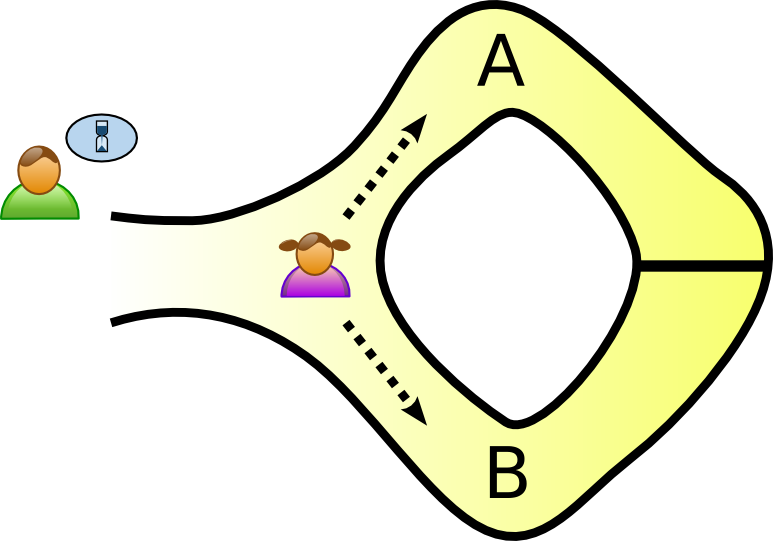
\includegraphics[width=0.3\textwidth]{Zkip_alibaba1.png}}
    \hfill
    \subfigure[Étape 2]{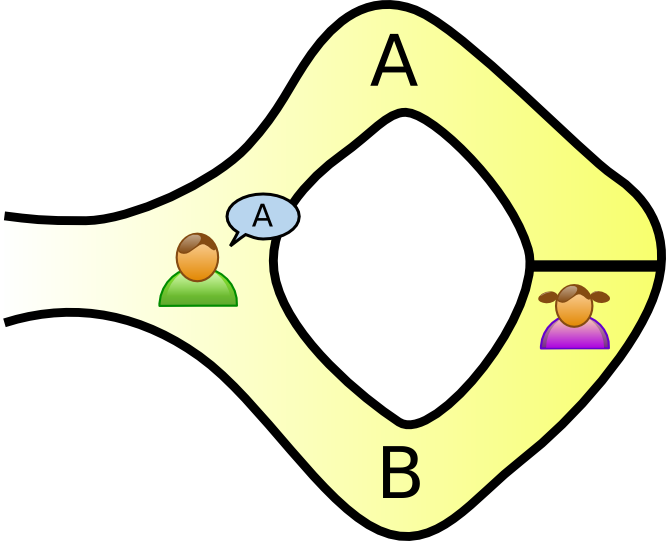
\includegraphics[width=0.3\textwidth]{Zkip_alibaba2.png}}
    \hfill
    \subfigure[Étape 3]{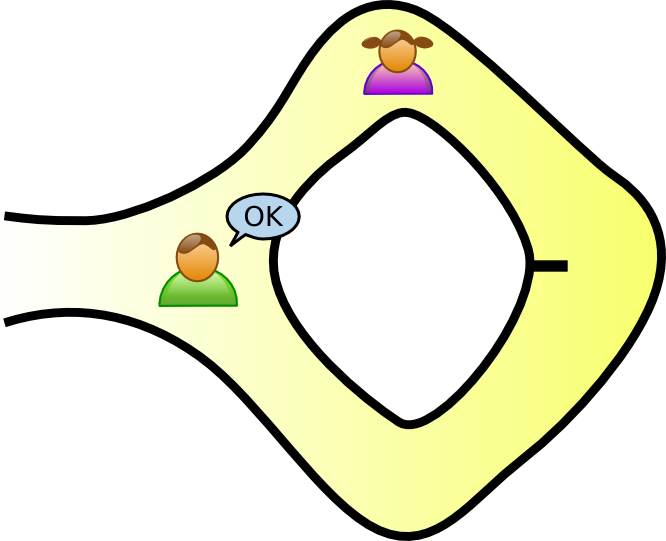
\includegraphics[width=0.3\textwidth]{Zkip_alibaba3.png}}
    \caption{Illustration du protocole Zero-Knowledge avec la grotte d'Ali Baba}
\end{figure}



\paragraph{Protocole.} Le protocole se déroule en plusieurs tours identiques:
\begin{enumerate}
    \item \textbf{Engagement \--\ (a)} : Peggy entre seule dans la grotte, en choisissant aléatoirement l'entrée A ou B.
    \item \textbf{Défi \--\ (b)} : Victor, qui reste à l'extérieur, crie « A » ou « B », demandant à Peggy de ressortir par l'une des deux entrées.
    \item \textbf{Réponse \--\ (c)} : 
    \begin{itemize}
        \item Si Peggy connaît le mot magique, elle peut ressortir par n'importe quelle sortie, même si elle doit passer par la porte.
        \item Si elle ne le connaît pas, elle ne pourra satisfaire la requête de Victor que si celui-ci demande la sortie correspondant à sa position initiale.
    \end{itemize}
\end{enumerate}

\paragraph{Interprétation.} Si Peggy ne connaît pas le mot magique, 
elle ne peut réussir le test que dans 50\,\% des cas. 
En répétant l'expérience plusieurs fois, Victor peut devenir 
presque certain que Peggy possède le mot magique. En effet, 
la probabilité qu'elle réussisse par pur hasard $N$ fois de suite 
est $\left(\frac{1}{2}\right){}^N$.

\paragraph{Conclusion.} Cette interaction permet à Victor de 
\textbf{vérifier que Peggy connaît le secret}, sans jamais 
apprendre quoi que ce soit sur le mot magique lui-même. 
Ce principe est à la base des Zero-Knowledge Proofs, qui sont 
largement utilisés en cryptographie moderne pour prouver des 
identités, des calculs ou des connaissances, sans rien dévoiler 
d'autre que la validité de l'affirmation.

\vspace{0.5cm}

Dans notre cas, cela permet de prouver le calcul de notre borne de latence,
sans avoir à divulguer une quelconque information sur le réseau utilisé.

\section*{Utilité des preuves}

Dans un contexte décentralisé, où les acteurs ne se font pas nécessairement confiance, la génération de preuve devient un outil clé pour établir une confiance automatisée et vérifiable.

Imaginons un scénario typique impliquant trois entités:
\begin{itemize}
    \item \textbf{Le client}, qui souhaite transmettre des données à travers un réseau avec des garanties strictes sur les délais.
    \item \textbf{L'opérateur}, chargé de configurer et de superviser le réseau.
    \item \textbf{La blockchain}, qui héberge une application décentralisée : un contrat intelligent jouant le rôle d'arbitre automatisé.
\end{itemize}

L'enjeu est simple : comment le client peut-il s'assurer que l'opérateur a bien configuré le réseau de façon à respecter les délais annoncés, sans pour autant avoir accès à tous les détails (souvent confidentiels) de la topologie ou de la charge du réseau?

\bigskip

\begin{center}
  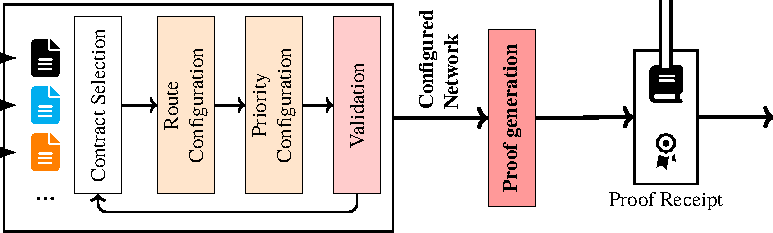
\includegraphics[width=0.9\textwidth]{main_cropped.pdf}
\end{center}

C'est ici que la \textbf{génération de preuve} entre en jeu.

\begin{itemize}
    \item L'opérateur exécute l'algorithme TFA, pour évaluer si les contraintes de latence sont respectées.
    \item Il génère ensuite une preuve, qui atteste que ce calcul a été effectué de manière honnête.
    \item Cette preuve est publiée sur la blockchain, pour que l'ensemble des acteurs puissent vérifier sa validité.
    \item Le contrat intelligent vérifie automatiquement la validité de cette preuve.
\end{itemize}

\medskip

En résumé, la génération de preuve permet de transformer une promesse (``je respecte les délais'') en une garantie vérifiable et infalsifiable. C'est un composant essentiel pour automatiser la confiance dans les systèmes distribués critiques, en s'appuyant sur des preuves objectives plutôt que sur des déclarations ou une surveillance constante.

\medskip

Ayant désormais un contexte sur l'utilité des bornes de latences
et de la génération de preuve à divulgation nulle de connaissances,
nous pouvons désormais nous concentrer sur l'objectif principal de
mon stage, l'optimisation de la génération de ces dites preuves.

% --------- Activités réalisées ---------
\chapter{Travaux effectués}

Le temps requis pour générer une preuve d'exécution est directement lié au nombre
de cycles de l'algorithme.
Nous cherchons donc à réduire ce nombre afin d'accélérer le processus de
génération.

\section{Optimisations pour une machine virtuelle}

\subsection{Profilage de code}

Le profilage de code est une étape essentielle dans le processus 
d'optimisation d'un programme informatique. Il consiste à analyser 
l'exécution du programme afin d'identifier les parties les plus 
coûteuses en ressources, telles que le temps de calcul ou la 
mémoire utilisée.

\medskip

Cette analyse permet de repérer les `goulots d'étranglement', 
c'est-à-dire les sections du code qui ralentissent 
globalement l'exécution. Grâce à ces informations, il 
est possible de concentrer les efforts d'optimisation sur 
ces portions spécifiques, maximisant ainsi l'amélioration 
des performances.

\medskip

Pour argumenter et discuter des différentes optimisations à réaliser,
nous allons nous appuyer sur cet outil, mais notamment sur la documentation
de `Risc Zero' (la machine virtuelle utilisée pour la génération de ZKPs), informant
sur des optimisations divergentes des optimisations sur des processeurs d'ordinateur classiques.

\subsection{Conversion des flottants vers des entiers}

Une première amélioration, non visible par profilage, est l'utilisation
d'entiers à la place de flottants. Dans une machine virtuelle, comme celle de 
\textbf{RISC Zero}, le choix du type de données utilisées au sein
du code à un impact significatif sur ses performances. Plus 
précisément, d'après la documentation de RISC Zero, les opérations 
sur des \textbf{entiers} sont plus efficaces que celles sur les \textbf{nombres flottants}. 

En effet, la machine virtuelle de RISC Zero n'inclut pas les
instructions pour le calcul en virgule flottante. Cela signifie
qu'elle ne sait pas exécuter directement les opérations
comme l'addition de flottants.

\medskip

Puisqu'il n'y a pas de prise en charge directe, toutes les opérations
flottantes sont simulées en logiciel. Cela veut dire que, pour effectuer
une opération flottante, la machine virtuelle doit exécuter
une série d'instructions entières qui imitent le comportement d'une addition
en virgule flottante.

\medskip

En conséquence, une opération entière prendra seulement 1 à 2
cycles, alors qu'une opération flottante consommera 60 à 140 cycles,
soit 30 à 100 fois plus de temps.

\medskip

\begin{figure}[h!]
\centering
\begin{tikzpicture}[
    box/.style = {rectangle, draw, rounded corners, minimum height=1cm, minimum width=3.5cm, align=center},
    arrow/.style = {->, thick},
    cycle/.style = {font=\small}
]

% Integer path
\node[box, fill=green!20] (intop) {Opération entière};
\node[box, fill=green!10, below=of intop] (intcycle) {1–2 cycles};
\draw[arrow] (intop) -- (intcycle);

% Float path
\node[box, fill=red!20, right=6cm of intop] (floatop) {Opération flottante};
\node[box, fill=red!10, below=of floatop] (floatsim) {Émulée en logiciel};
\node[box, fill=red!10, below=of floatsim] (floatcycle) {60–140 cycles};

\draw[arrow] (floatop) -- (floatsim);
\draw[arrow] (floatsim) -- (floatcycle);

% Comparison arrow
\draw[thick, dashed, <->] (intcycle.east) -- node[cycle, above, align=center] {30–100× \\ plus coûteux} (floatcycle.west);

% Labels
\node[font=\bfseries, above=0.5cm of intop] {Entiers};
\node[font=\bfseries, above=0.5cm of floatop] {Flottants};

\end{tikzpicture}
\end{figure}

\medskip

Cependant, l'utilisation d'entiers n'est pas sans compromis:
si l'addition, la soustraction et la multiplication ne sont pas 
des problèmes avec ce type de données, la division en est une.
En Rust, une division d'entiers est performé en tronquant sa partie
décimale. Par exemple, si avec des flottants $1.0/2.0 = 0.5$,
avec des entiers $1/2 = 0$. Malheureusement, on calcule des bornes de
latences, on ne peut pas se permettre de sur-estimer cette dernière
en tronquant systématiquement la partie décimale.

\medskip

Pour pallier ce problème, il a fallu dans un premier temps convertir
l'ensemble des données en entrées sur une unité plus faible pour 
conserver la précision apporté par leurs parties décimales (ex: 
$3.5$ms $=$ $3500$µs) puis créer une fonction réalisant une
division entière en arrondissant à l'entier supérieur. ($1/2 = 1$).
Dû au changement d'unité, la perte induit par l'arrondi est négligeable.

\subsection{Optimisation des structures de données}

\begin{center}
  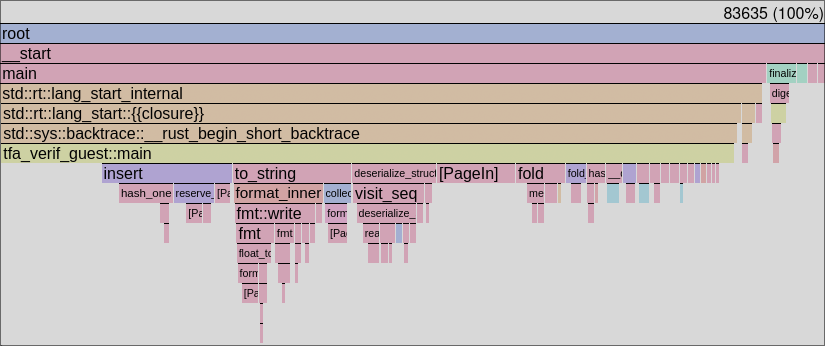
\includegraphics[width=1\textwidth]{flamegraph_1.png}
\end{center}

En étudiant le profilage du code, présent ci-dessus, on observe
qu'une importante partie des cycles totaux est dû aux insertions
(dû au bloc `insert', étant le bloc le plus à gauche dans le profilage) 
dans nos structures de données: la HashMap et le HashSet.

\medskip

La \textit{HashMap} associe des clés à des valeurs en utilisant 
une table de hachage. Chaque clé est transformée par une fonction 
de hachage en un indice qui indique où stocker la valeur. Cela 
permet un accès rapide, mais le calcul du hachage peut être coûteux.

\vspace{0.3cm}
\begin{center}
\begin{tikzpicture}[
  node distance=0.8cm,
  box/.style={rectangle, draw, minimum width=3cm, minimum height=1cm, align=center},
  arrow/.style={->, thick}
]
\node[box] (key) {Clé};
\node[box, right=of key] (hash) {Calcul du hash};
\node[box, right=of hash] (bucket) {Emplacement};
\node[box, below=of bucket] (value) {Valeur};
\draw[arrow] (key) -- (hash);
\draw[arrow] (hash) -- (bucket);
\draw[arrow] (bucket) -- (value);
\end{tikzpicture}
\end{center}

\vspace{0.3cm}

Le \textit{HashSet} stocke uniquement des éléments uniques, 
sans valeurs associées. Il utilise aussi une table de hachage 
pour déterminer la position de chaque élément. Le fonctionnement 
est donc similaire au HashMap, mais sans la valeur.

\vspace{0.3cm}
\begin{center}
\begin{tikzpicture}[
  node distance=1.5cm,
  circleNode/.style={circle, draw, minimum size=1.2cm, align=center},
  arrow/.style={->, thick}
]
\node[circleNode] (elem) {Élément};
\node[box,fill=white, right=of elem] (hash) {Calcul du hash};
\node[box,fill=white, right=of hash] (bucket) {Emplacement};
\draw[arrow] (elem) -- (hash);
\draw[arrow] (hash) -- (bucket);
\end{tikzpicture}
\end{center}

\vspace{0.3cm}

En regardant plus en profondeur le profilage, on remarque que ce qui
est couteux durant les insertions est le hachage effectué sur la clé (HashMap)
ou l'élément (HashSet). Pour éviter ce coût élevé en cycle, la documentation
de RISC Zero recommande d'utiliser des BTreeMap et des BTreeSet.

\medskip

La \textit{BTreeMap} organise les clés et valeurs dans un arbre 
équilibré. Les clés sont conservées dans un ordre trié et les 
accès se font par comparaison (plus petit → à gauche, plus grand →
à droite). Il n'y a pas de calcul de hachage, 
ce qui réduit certains coûts.

\vspace{0.3cm}
\begin{center}
\begin{tikzpicture}[
  level distance=1.75cm,
  sibling distance=3cm,
  every node/.style={draw, rectangle, minimum width=2.5cm, minimum height=1cm, align=center},
  edge from parent/.style={draw, -latex}
]
\node {Clé 50}
  child {node {Clé 20 \\ Valeur A}}
  child {node {Clé 80 \\ Valeur B}};
\end{tikzpicture}
\end{center}

\vspace{0.3cm}

Le \textit{BTreeSet} stocke des éléments uniques dans un arbre 
équilibré. Les éléments sont triés et les opérations utilisent 
la comparaison sans hachage.

\vspace{0.3cm}
\begin{center}
\begin{tikzpicture}[
  level distance=1.2cm,
  sibling distance=3cm,
  every node/.style={draw, circle, minimum size=1.5cm, align=center},
  edge from parent/.style={draw, -latex}
]
\node {B}
  child {node {A}}
  child {node {C}};
\end{tikzpicture}
\end{center}

\medskip

En remplaçant l'intégralité des HashMap et des HashSet par des
BTreeMap et des BTreeSet, on réduit considérablement le coût
des insertions en supprimant l'utilisation de fonctions de
hachage.

\medskip

La réalisation d'un deuxième profilage, présent ci-dessous, vient confirmer la réduction
du nombre total de cycles (voir en haut à droite), mais notamment
la réduction du nombre de cycles dû aux insertions (absence du bloc
`insert' présent dans le profilage précédent).

\begin{center}
  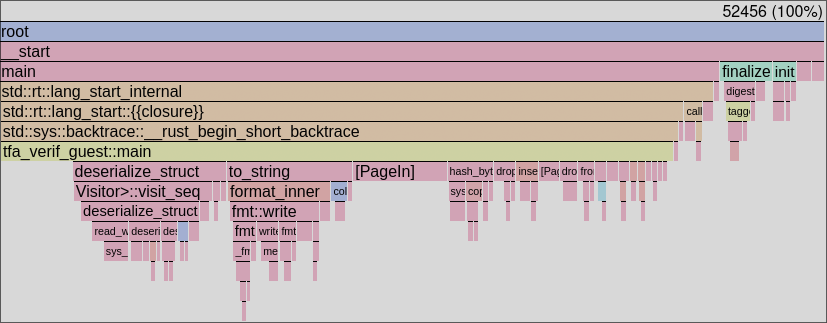
\includegraphics[width=1\textwidth]{flamegraph_2.png}
\end{center}

\break{}

\subsection{Changement de fonction de hachage}

Lors du profilage précédent, deux blocs importants restent 
visibles~: \texttt{deserialize\_struct} et \texttt{to\_string}. 
Le premier, indispensable, correspond à la lecture d'un fichier 
\texttt{JSON} par notre code, permettant de récupérer la topologie 
du réseau ainsi que les différents contrats le traversant.

\medskip

En revanche, le bloc \texttt{to\_string} peut être optimisé. Cette 
instruction correspond à la conversion des contrats validés par 
l'algorithme en chaînes de caractères, en vue de leur hachage 
pour un envoi sécurisé.

\medskip

En remplaçant cette conversion par l'utilisation directe de 
la fonction de hachage native de RISC Zero, on peut supprimer 
l'étape intermédiaire de transformation en chaîne de caractères. 
Cette optimisation permet de réduire significativement le nombre 
de cycles nécessaires au hachage des contrats validés de par la 
suppression des cycles dû à la conversion.

\begin{center}
\begin{tikzpicture}[
  node distance=1.5cm and 2cm,
  every node/.style={font=\small},
  box/.style={draw, rectangle, rounded corners, minimum height=1cm, minimum width=2.8cm, align=center},
  arrow/.style={-{Latex[length=2mm]}, thick}
]

% First row (Before)
\node[box] (contracts1) {Contrats validés};
\node[box, right=of contracts1] (stringify) {Conversion \\ \texttt{to\_string}};
\node[box, right=of stringify] (hash1) {Hachage};

% Second row (After)
\node[box, below=2.2cm of contracts1] (contracts2) {Contrats validés};
\node[box, right=3.8cm of contracts2] (hash2) {Hachage natif \\ RISC Zero};

% Arrows (Before)
\draw[arrow] (contracts1) -- (stringify);
\draw[arrow] (stringify) -- (hash1);

% Arrows (After)
\draw[arrow] (contracts2) -- (hash2);

% Labels
\node[above=0.2cm of contracts1, font=\bfseries] {Avant optimisation};
\node[above=0.2cm of contracts2, font=\bfseries] {Après optimisation};

\end{tikzpicture}
\end{center}

Ci-dessous, le profilage final avec l'ensemble des modifications
apportées, montrant ainsi une diminution importante du nombre total
de cycles (83635 → 46433, soit 1,8x plus rapide).

\begin{center}
  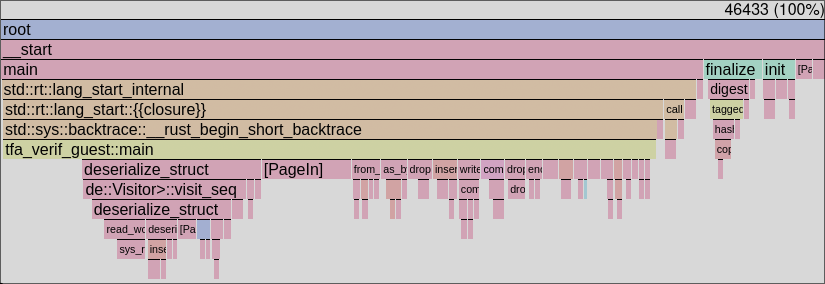
\includegraphics[width=1\textwidth]{flamegraph_3.png}
\end{center}

\break{}
\section{Optimisations structurelles}

Si les optimisations précédentes était spécifiques à la machine
virtuelle de RISC Zero, les optimisations structurelles, elles, sont
indépedantes de la plateforme d'exécution est profitable pour
n'importe quel environnement. 

\medskip

Elles visent à transformer le code source afin de le rendre plus
efficace en termes de structure logique ou de complexité
algorithmique. Cela inclut, par exemple, l'élimination de code non
utilisé, la simplification d'expressions, ou encore la réduction
du nombre d'itérations dans des boucles.

\medskip

Parmi la liste des optimisations structurelles effectuées sur 
le code originel, la majorité permettent surtout une meilleure 
lisibilité du code en lui-même (notamment en utilisant de la
programmation fonctionnelle). On retrouve cependant deux changements majeurs dans le code
reflétant une accélération non négligeable.

\medskip

La première est la réduction du nombre de variables initialisées
au sein du code. Créer une variable implique une allocation en 
registre ou en mémoire. Chaque écriture ou lecture d'une variable
coûte ainsi des cycles supplémentaires. Travailler directement
sur les données en évitant au maximum la création de variables 
intermédiaires, permet de réduire considérablement le nombre de cycles.
Ci-dessous un exemple de code non optimisé et optimisé en réduisant
le nombre de créations de variables.

\smallskip

\begin{center}
\begin{tikzpicture}[
  node distance=1.2cm and 3cm,
  process/.style={rectangle, draw=black, rounded corners, minimum width=4.8cm, minimum height=1cm, align=center},
  comment/.style={rectangle, draw=gray, fill=gray!10, rounded corners, minimum width=5cm, align=left, font=\small},
  arrow/.style={-{Latex}, thick}
]

% Version verbeuse
\node[draw=none] (before) {\textbf{Code non optimisé}};
\node[process, below=of before] (v1) {let a = x + 1};
\node[process, below=of v1] (v2) {let b = a * 2};
\node[process, below=of v2] (v3) {let c = b - 3};
\node[process, below=of v3] (vres) {Résultat final = c};

\draw[arrow] (v1) -- (v2);
\draw[arrow] (v2) -- (v3);
\draw[arrow] (v3) -- (vres);

% Version optimisée
\node[draw=none, right=4cm of before] (after) {\textbf{Code optimisé}};
\node[process, below=of after] (opt1) {let res = ((x + 1) * 2) - 3};
\node[process, below=of opt1] (opt2) {Résultat final = res};

\node[comment, below=3cm of opt1] (comment2) {
Le calcul est direct.\\
Moins de variables intermédiaires.\\
Moins d'instructions à exécuter.\\
Exécution plus rapide et plus efficace.
};

\draw[arrow] (opt1) -- (opt2);

\end{tikzpicture}
\end{center}

\medskip

La deuxième amélioration, en lien avec la première, consiste à sauvegarder
des calculs déjà effectués et qui sont destinés à être réutilisés par la
suite. Regardons plus en détails les deux optimisations possibles 
dans l'algorithme.

\subsection*{Somme des bursts de priorités supérieures $\sum_{c'>c} b^c_n$}

\begin{center}
\begin{minipage}{0.47\textwidth}
\raggedright{}
Le principe est que pour une classe de priorité $c$, à un nœud du
réseau $n$, on additionne les bursts arrivant à ce nœud seulement
pour les classes de priorités supérieures à celle sur laquelle on
se positionne.

\medskip

Originellement, on recalculait cette somme pour chaque classe de 
priorité. Cependant, de par le fait que l'on commence à la classe 
de priorité la plus élevée, nous pouvons stocker au fur et à mesure
le burst de la classe calculé pour pouvoir le réexploiter dans le
calcul de la somme des bursts de priorités supérieures.

\medskip

Ci-contre un schéma synthétisant la nouvelle méthode du calcul
de la somme des bursts de priorités supérieures.
\end{minipage}%
\hfill
\begin{minipage}{0.48\textwidth}
\centering
\begin{tikzpicture}[scale=0.7, transform shape,
  node distance=1cm and 2.8cm,
  process/.style={rectangle, draw=black, rounded corners, minimum width=3cm, minimum height=1cm, align=center},
  storage/.style={rectangle, draw=blue, minimum width=2.5cm, minimum height=0.8cm, fill=blue!10},
  arrow/.style={-{Latex}, thick}
]

\node[draw=none] (before) {\textbf{Avant}};

\node[process, align=center, below=of before] (naive_start) {Calculer le burst\\ de la classe $c$};
\node[process, below=of naive_start] (naive_sum) {Recalculer $\sum_{c'>c} b^c_n$};
\node[process, below=of naive_sum] (naive_compute) {Suite des calculs ...};

\draw[arrow] (naive_start) -- (naive_sum);
\draw[arrow] (naive_sum) -- (naive_compute);

\node[draw=none, right=4cm of before] (after) {\textbf{Après}};

\node[process, align=center, below=of after] (opt_start) {Calculer le burst\\ de la classe $c$};
\node[storage, below=of opt_start] (opt_compute) {Stocker résultat pour la classe $c$};
\node[storage, below=of opt_compute] (opt_reuse) {Réutiliser $\sum_{c'>c} b^c_n$};
\node[process, below=of opt_reuse] (opt_store) {Suite des calculs ...};

\draw[arrow] (opt_start) -- (opt_compute);
\draw[arrow] (opt_compute) -- (opt_reuse);
\draw[arrow] (opt_reuse) -- (opt_store);

\end{tikzpicture}
\end{minipage}
\end{center}

\medskip

\subsection*{Somme des rates de priorités supérieures $\sum_{c'>c} r^c_n$}

\begin{center}
\begin{minipage}{0.47\textwidth}
\raggedright{}
La deuxième optimisation consiste à réaliser un raisonnement analogue
à la somme des bursts de priorités supérieures, mais cette fois-ci
pour le rate.

\medskip

Ci-contre un schéma synthétisant la méthode du calcul
de la somme des rates de priorités supérieures, analogue à celle
des bursts.
\end{minipage}%
\hfill
\begin{minipage}{0.48\textwidth}
\centering
\begin{tikzpicture}[scale=0.7, transform shape,
  node distance=1cm and 2.8cm,
  process/.style={rectangle, draw=black, rounded corners, minimum width=3cm, minimum height=1cm, align=center},
  storage/.style={rectangle, draw=blue, minimum width=2.5cm, minimum height=0.8cm, fill=blue!10},
  arrow/.style={-{Latex}, thick}
]

\node[draw=none] (before) {\textbf{Avant}};

\node[process, align=center, below=of before] (naive_start) {Calculer le rate\\ de la classe $c$};
\node[process, below=of naive_start] (naive_sum) {Recalculer $\sum_{c'>c} b^c_n$};
\node[process, below=of naive_sum] (naive_compute) {Suite des calculs ...};

\draw[arrow] (naive_start) -- (naive_sum);
\draw[arrow] (naive_sum) -- (naive_compute);

\node[draw=none, right=4cm of before] (after) {\textbf{Après}};

\node[process, align=center, below=of after] (opt_start) {Calculer le rate\\ de la classe $c$};
\node[storage, below=of opt_start] (opt_compute) {Stocker résultat pour la classe $c$};
\node[storage, below=of opt_compute] (opt_reuse) {Réutiliser $\sum_{c'>c} b^c_n$};
\node[process, below=of opt_reuse] (opt_store) {Suite des calculs ...};

\draw[arrow] (opt_start) -- (opt_compute);
\draw[arrow] (opt_compute) -- (opt_reuse);
\draw[arrow] (opt_reuse) -- (opt_store);

\end{tikzpicture}
\end{minipage}
\end{center}

\bigskip

Les dernières optimisations réalisées marquant la fin de cette
partie sont des optimisations propres au compilateur de Rust,
appelé \texttt{rustc}, elles sont presque négligeables et
n'ont pas d'intérêts à être développées dans ce rapport. 


% --------- Résultats ---------
\chapter{Évaluation des performances}
\section{Qu'est-ce qu'un benchmark?}

Un \textbf{benchmark} est un test ou un ensemble de tests 
standardisés permettant d'évaluer les performances d'un système, 
d'un programme ou d'un algorithme. Il permet de mesurer des 
métriques clés (comme le temps d'exécution, l'utilisation mémoire, 
etc.) en fonction de différents paramètres, afin de comparer, 
analyser ou améliorer une solution informatique.

\section*{Paramètres du benchmark}

Dans notre cas, le benchmark fait varier deux paramètres principaux:
\begin{itemize}
    \item \textbf{Le nombre de nœuds} dans le réseau ($n$), représentant la taille du système distribué.
    \item \textbf{Le nombre de contrats} (flux) ($c$) circulant dans le réseau.
\end{itemize}

Ces paramètres influencent directement la complexité du calcul 
des bornes, étant donné que le calcul des bornes de latences
à une complexité de $n*c$.

\section*{Mesures effectuées}

Pour chaque configuration $(n, c)$, on mesure:
\begin{itemize}
    \item la \textbf{nombre de cycles} enregistrés.
    \item le \textbf{temps d'exécution} du benchmark.
\end{itemize}

\begin{center}
\begin{tikzpicture}[node distance=1.8cm and 2cm, scale=0.95, transform shape, every node/.style={font=\small}]

    % Entrées
    \node[draw, fill=blue!10, rounded corners, minimum width=2.8cm, minimum height=1cm] (nodes) {Nombre de nœuds $n$};
    \node[draw, fill=blue!10, rounded corners, below of=nodes] (contracts) {Nombre de contrats $c$};

    % Algorithme
    \node[draw, fill=orange!20, rounded corners, right=of nodes, minimum width=4.5cm, minimum height=2.5cm] (algo) {
        \begin{tabular}{c}
            \textbf{Algorithme} \\
            Calcul des bornes \\
            de latence
        \end{tabular}
    };

    % Résultats
    \node[draw, fill=green!20, rounded corners, right=of algo, minimum width=4cm, minimum height=2cm] (output) {
        \begin{tabular}{l}
            $\bullet$ Nombre de cycles \\
            $\bullet$ Temps d'éxecution \\
        \end{tabular}
    };

    % Flèches
    \draw[->, thick] (nodes.east) -- (algo.west);
    \draw[->, thick] (contracts.east) -- (algo.west);
    \draw[->, thick] (algo.east) -- (output.west);

\end{tikzpicture}
\end{center}

\section{Résultats expérimentaux}

Comme dit précédemment, la complexité de l'algorithme TFA dépend
du nombre de nœuds comprenant le réseau, ainsi que le nombre de 
contrats les parcourant. 

Ci-dessous deux graphiques mettant en avant le nombre de cycles 
enregistrés, pour chaque optimisation discutées précédemment,
en faisant varier uniquement le nombre de nœuds ou le 
nombre de contrats.

\begin{figure}[H]
    \centering
    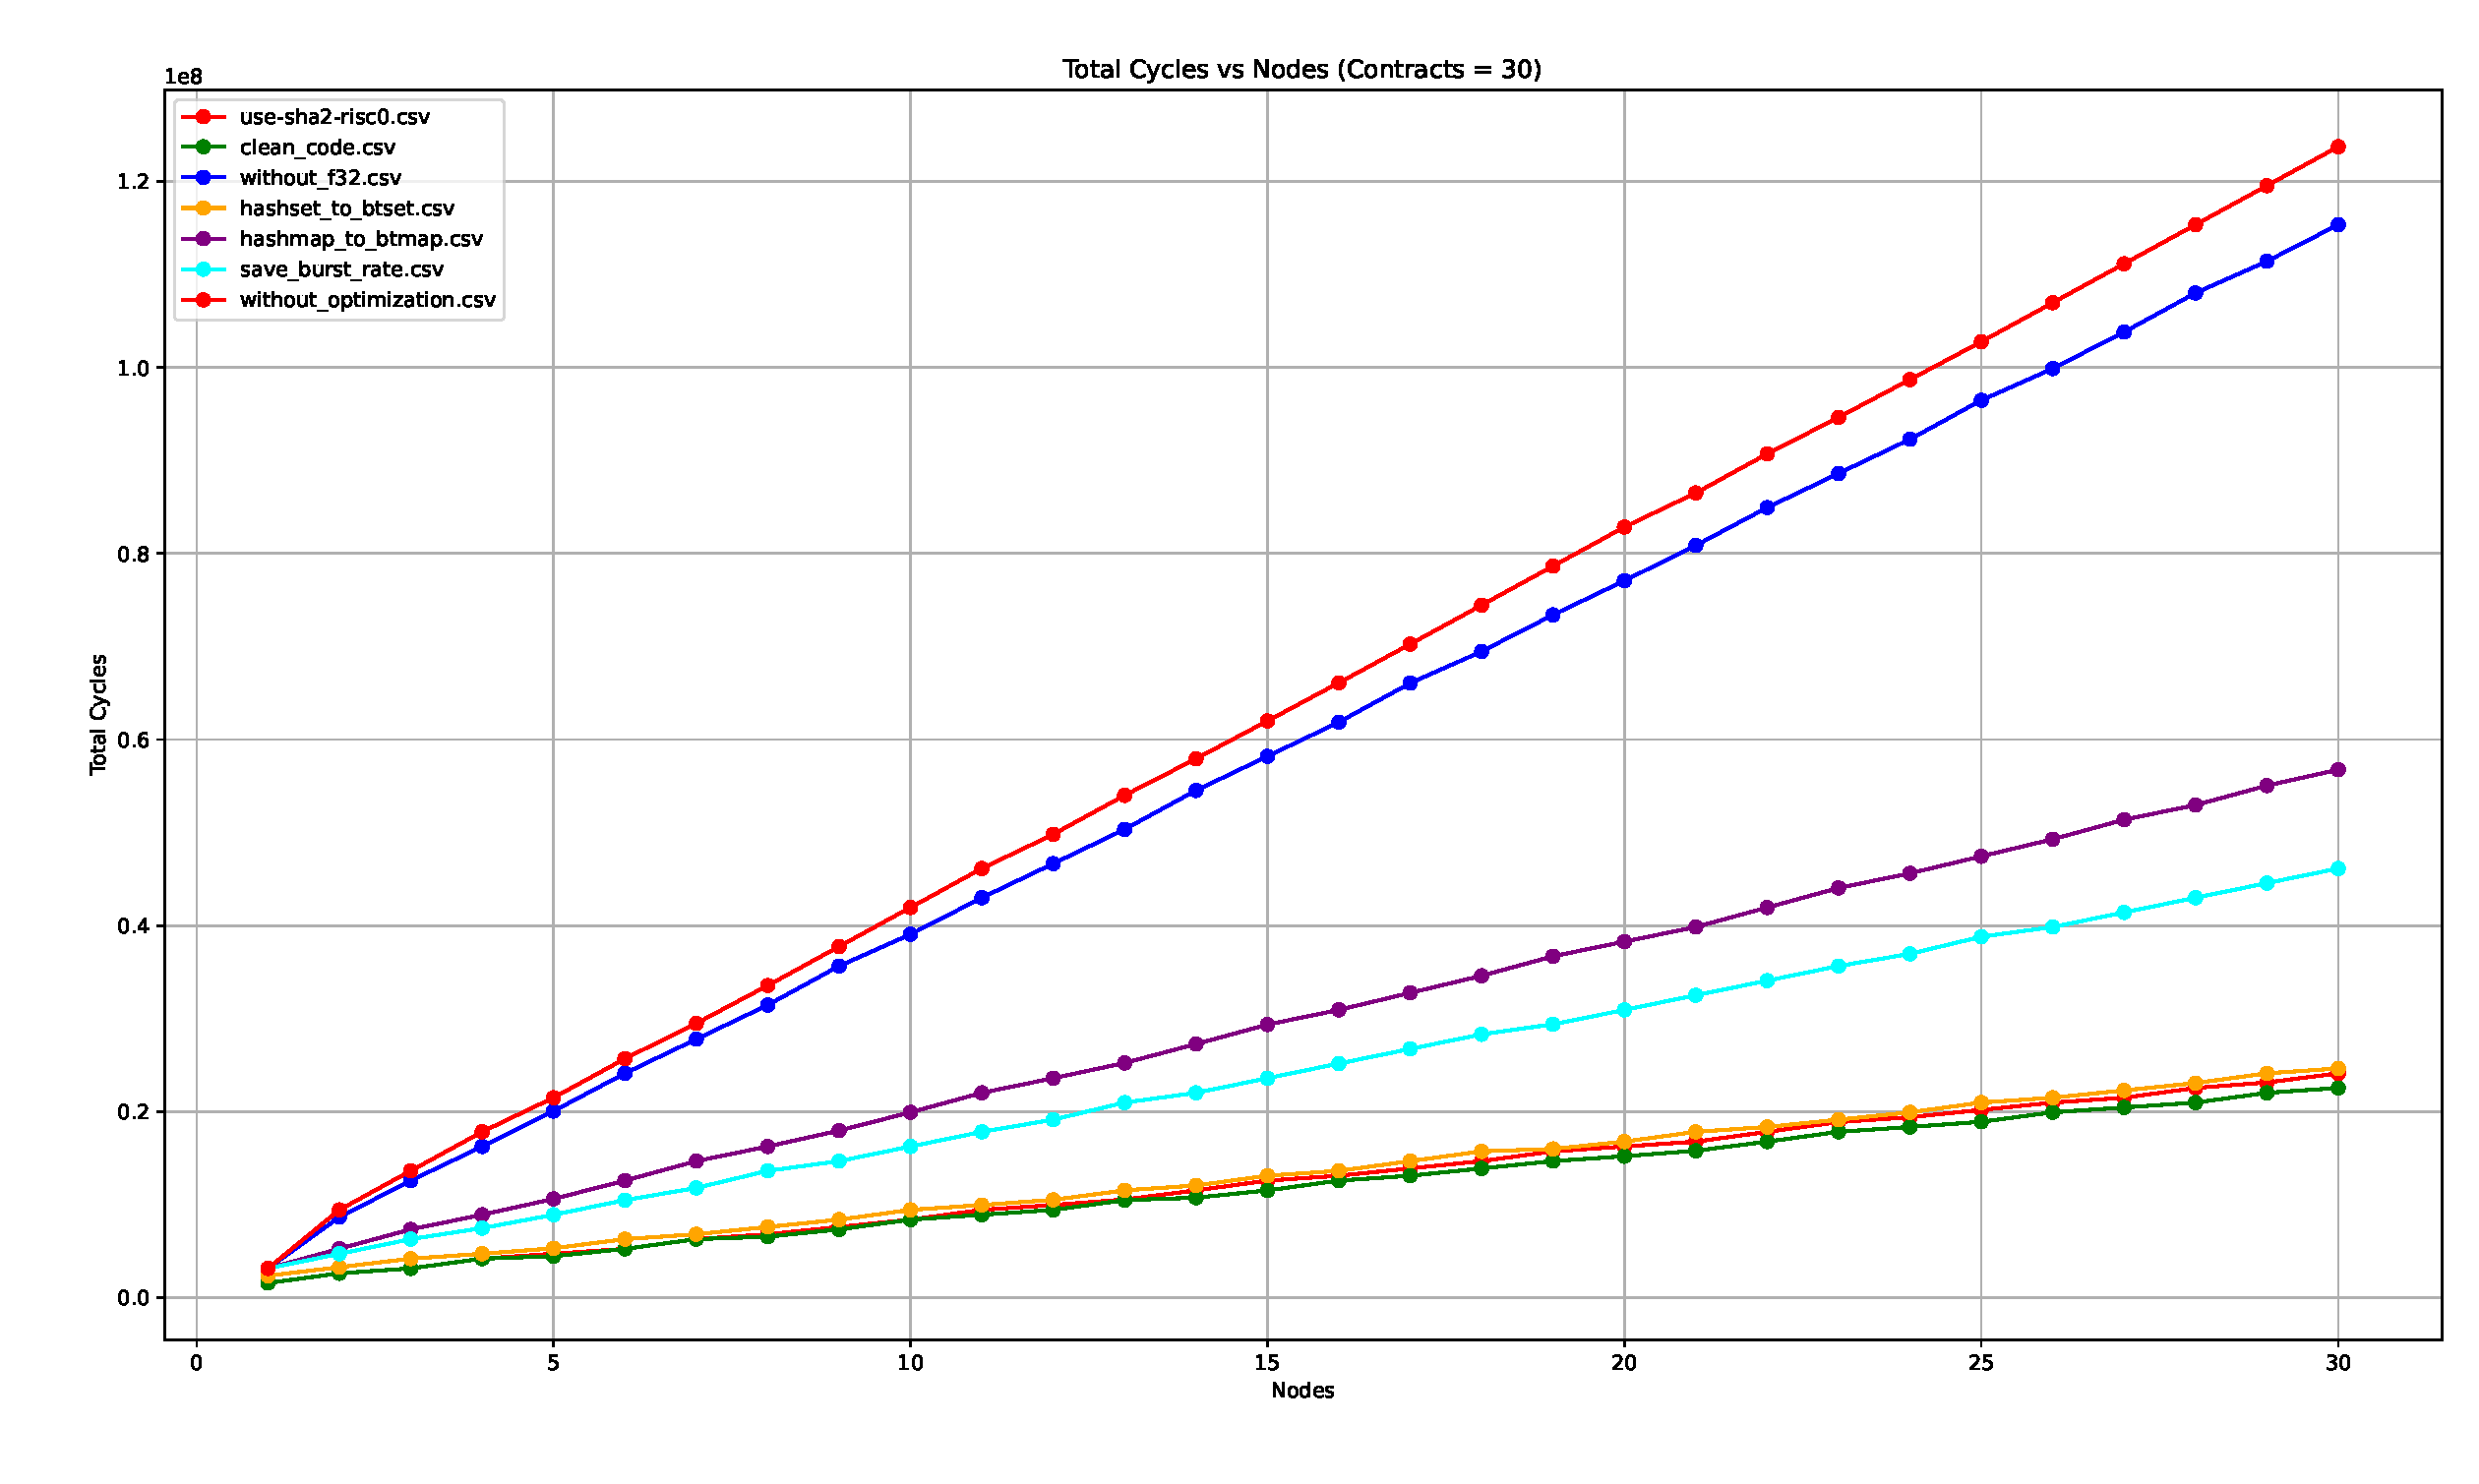
\includegraphics[width=0.9\textwidth]{benchmark_contracts.pdf}
    \caption{Temps de calcul des bornes de latences selon le nombre de nœuds}
    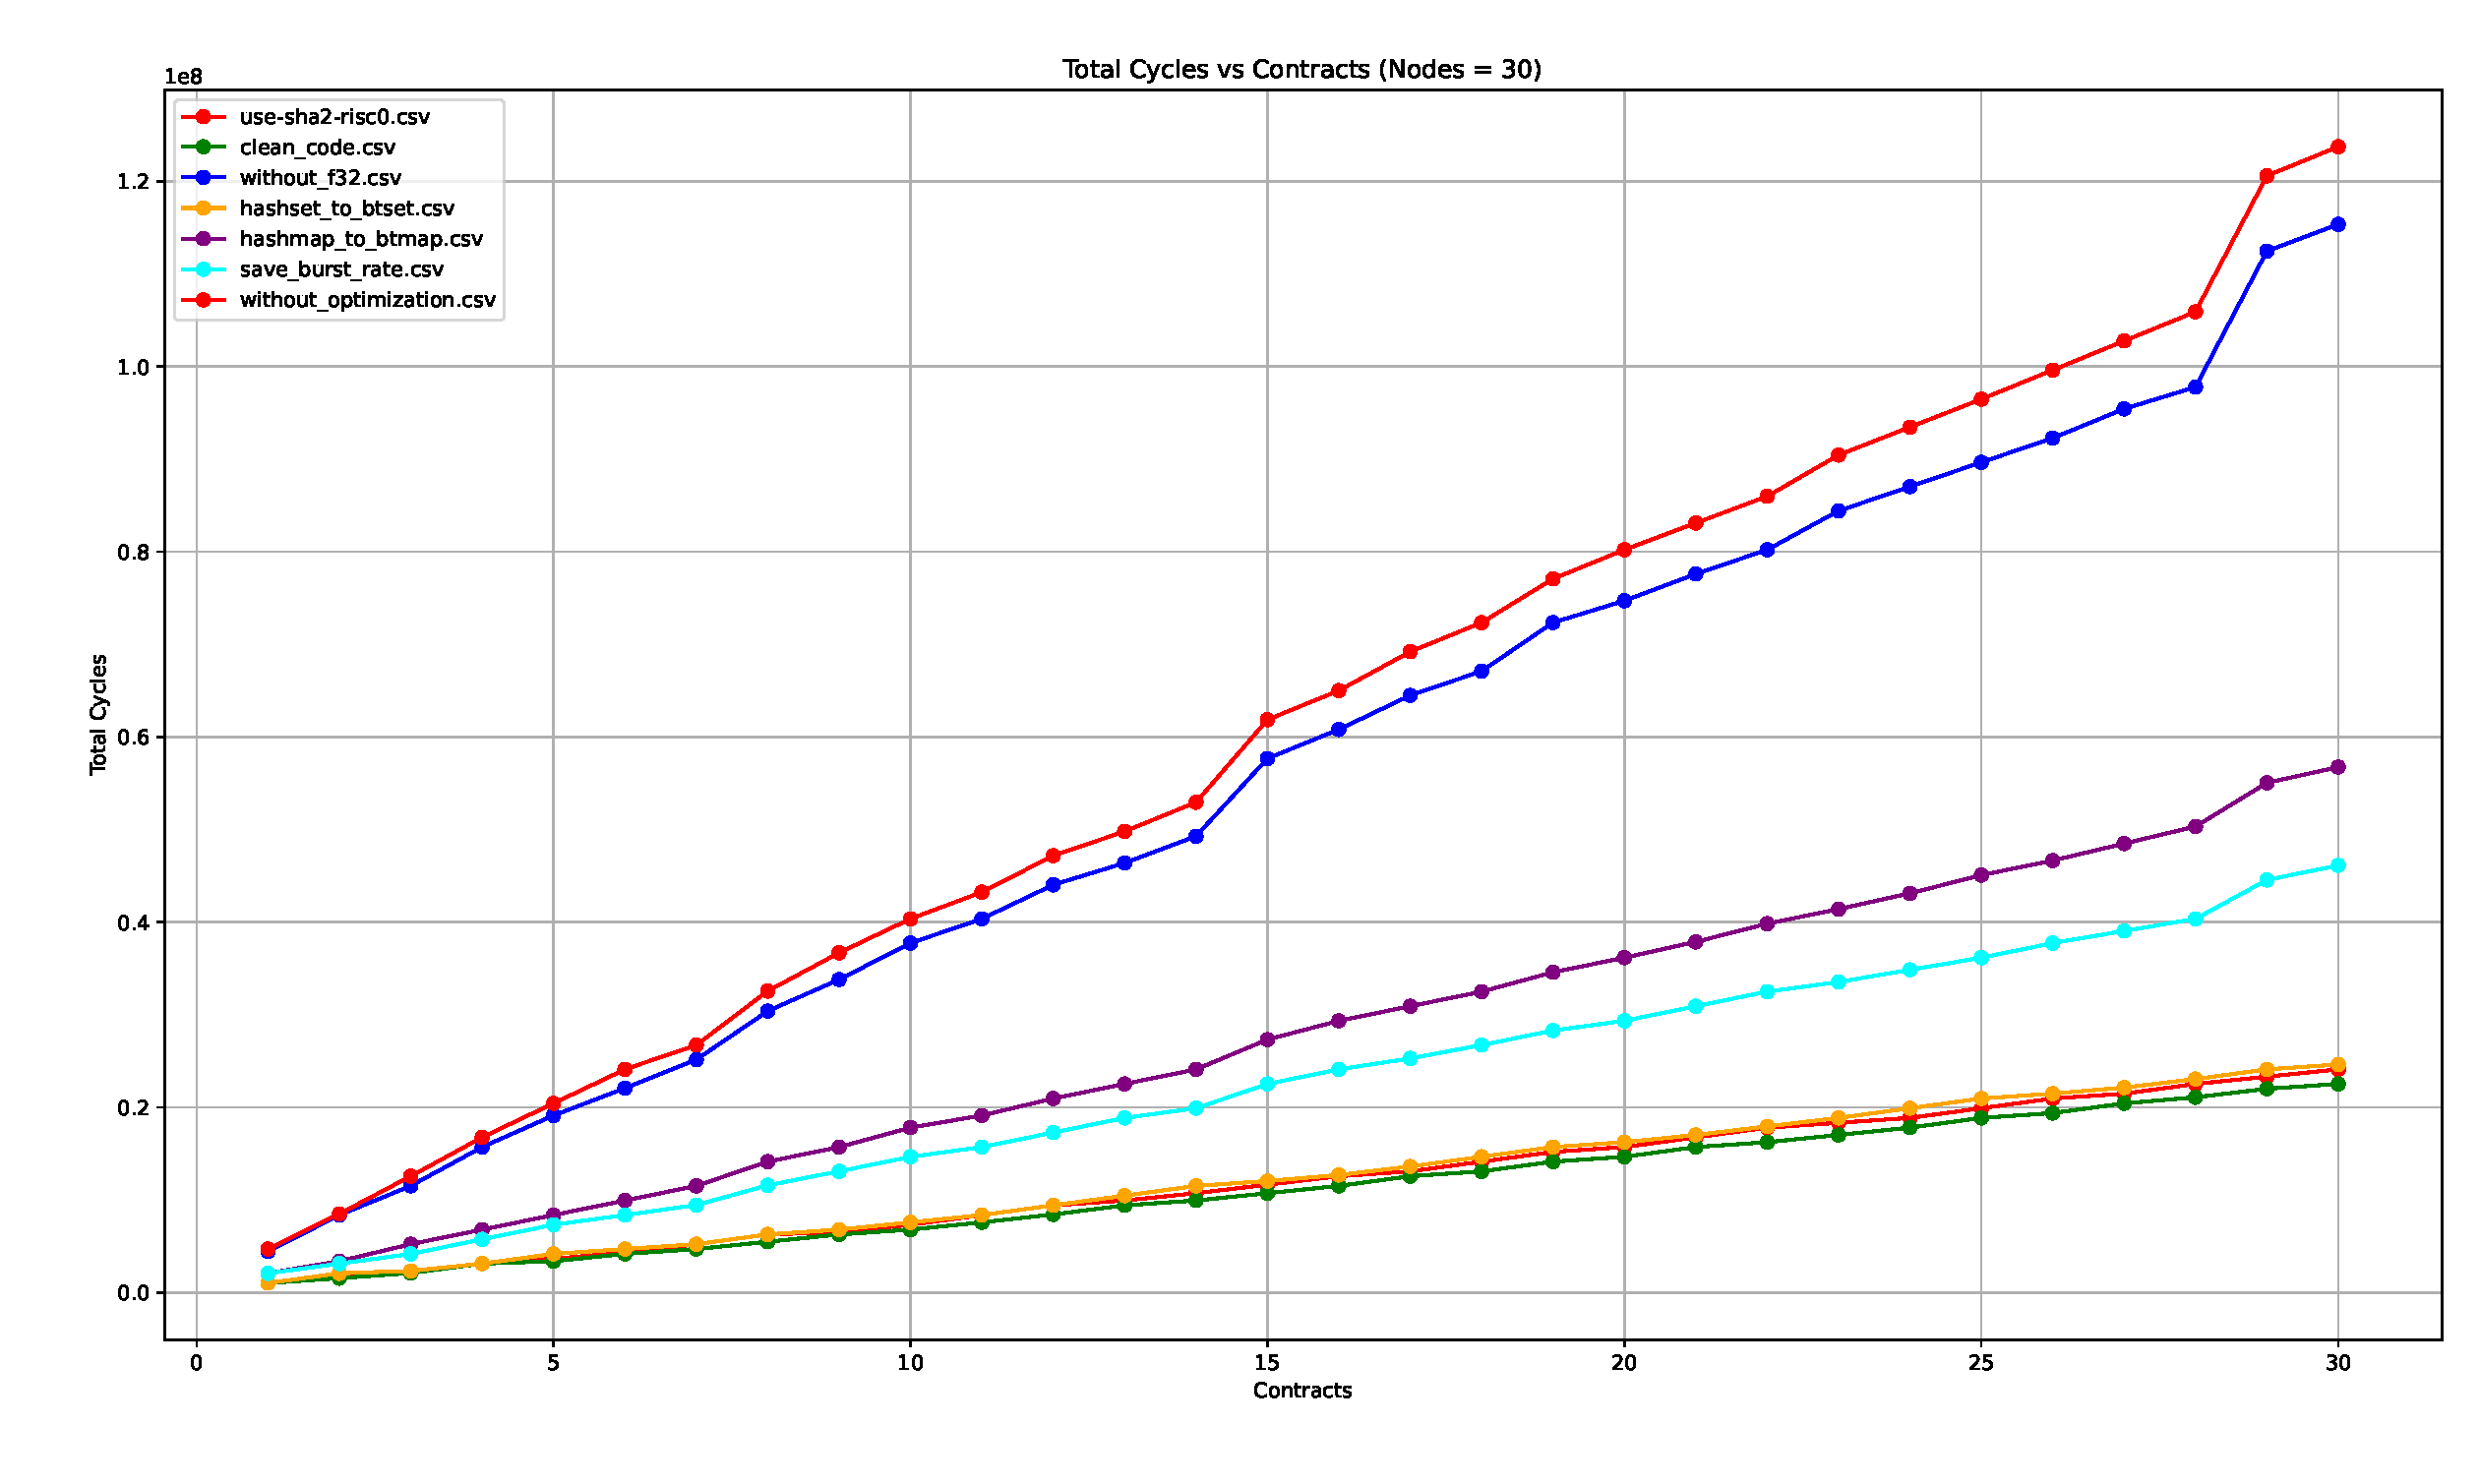
\includegraphics[width=0.9\textwidth]{benchmark_nodes.pdf}
    \caption{Temps de calcul des bornes de latences selon le nombre de contrats}
\end{figure}

\break{}

À noter que les différentes optimisations sont cumulatives, elles s'appuient sur les
précédentes.

\smallskip

Voici un rappel des optimisations correspondantes aux différentes courbes
présentent sur les deux graphiques:

\begin{center}
\begin{tikzpicture}
\begin{axis}[
    hide axis,
    xmin=0, xmax=1,
    ymin=0, ymax=1,
    legend style={
        draw=none,
        fill=none,
        nodes={scale=1, transform shape, anchor=west},
        at={(0,1)},
        anchor=north west,
        /tikz/column 2/.style={column sep=1em},
        align=left 
    }
]

\addlegendimage{color=red, mark=*}
\addlegendentry{\textbf{without\_optimization:} code initial, aucune optimisation}

\addlegendimage{color=blue, mark=*}
\addlegendentry{\textbf{without\_f32:} conversion de l'ensemble des flottants en entiers}

\addlegendimage{color=purple, mark=*}
\addlegendentry{\textbf{hashmap\_to\_btmap:} conversion de l'ensemble des HashMap en BTreeMap}

\addlegendimage{color=cyan, mark=*}
\addlegendentry{\textbf{save\_burst\_rate:} optimisation de la méthode de calcul du rate et du burst}

\addlegendimage{color=orange, mark=*}
\addlegendentry{\textbf{hashset\_to\_btset:} conversion de l'ensemble des HashSet en BTreeSet}

\addlegendimage{color=red, mark=*}
\addlegendentry{\textbf{use\_sha2\_risc0:} changement de fonction de hachage}

\addlegendimage{color=green!60!black, mark=*}
\addlegendentry{\textbf{clean\_code:} suppression de code redondant et inutilisé} 

\end{axis}
\end{tikzpicture}
\end{center}

On observe un gain important avec l'optimisations des structures de 
données utilisées au sein du code, ce qui est cohérent étant donné
leurs importantes présences.

L'échelle étant très importante ($1e8 = 100000000$ cycles), certaines
optimisations peuvent être discutables, mais elles apportent toutes
un gain de performance non négligeable.

Voici un tableau synthétisant l'ensemble des résultats de benchmark:

\bigskip

\begin{table}[h!]
\centering
\begin{tabular}{|l|r|r|r|}
\hline
\textbf{Optimisation} & \textbf{Cycles moyens} & \textbf{Accélération} & \textbf{Réduction (\%)} \\
\hline
without\_optimization.csv & 31941281.56 & 1.00x & 0.00\% \\
without\_f32.csv       & 29764448.71 & 1.07x & 6.82\%  \\
hashmap\_to\_btmap.csv & 14783811.13 & 2.16x & 53.72\% \\
save\_burst\_rate.csv  & 12123104.14 & 2.63x & 62.05\% \\
hashset\_to\_btset.csv &  6886004.05 & 4.64x & 78.44\% \\
use\_sha2\_risc0.csv   &  6505704.11 & 4.91x & 79.63\% \\
clean\_code.csv        &  6158727.40 & 5.19x & 80.72\% \\
\hline
\end{tabular}
\caption{Résultats de benchmark triés par ordre croissant de réduction des cycles}
\end{table}

\bigskip

Ci-dessous un diagramme en 3D mettant en opposition le code initial ainsi
que le code final afin d'étudier leurs complexités en faisant varier
à la fois le nombre de nœuds et le nombre de contrats.

\begin{figure}[H]
    \centering
    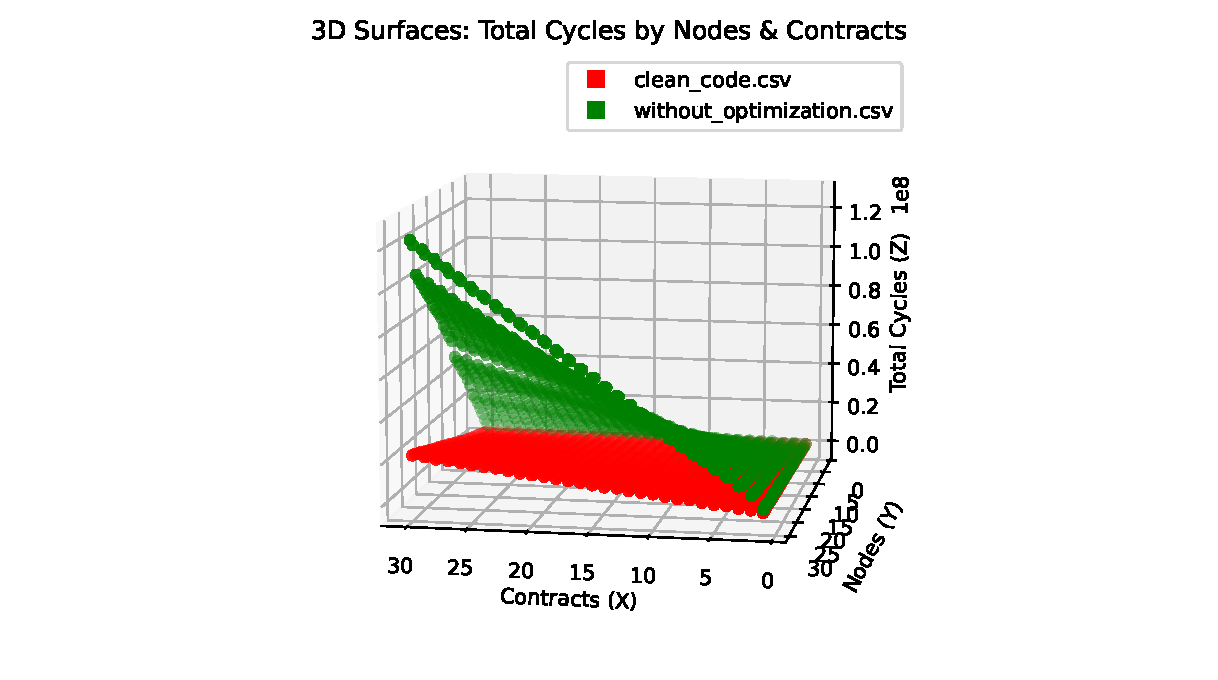
\includegraphics[width=0.95\textwidth]{benchmark_3D.pdf}
    \caption{Temps de calcul des bornes de latences selon le nombre de nœuds \textbf{et} le nombre de contrats}
\end{figure}

À noter que l'ensemble des benchmarks ont été fait sur un réseau paramétrique linéaire,
où le nombre de contrats et de nœuds sont variables. Ces benchmarks n'évaluent pas
leurs performances dans un contexte réaliste, mais permettent d'étudier le
comportement des différentes optimisations apportées au code.

\bigskip

Cependant, nous pouvons observer sur le graphique ci-dessous, que les optimisations sont 
encore valables sur un exemple de réseau industriel, où les contrats sont envoyés 
un par un.

\begin{figure}[H]
    \centering
    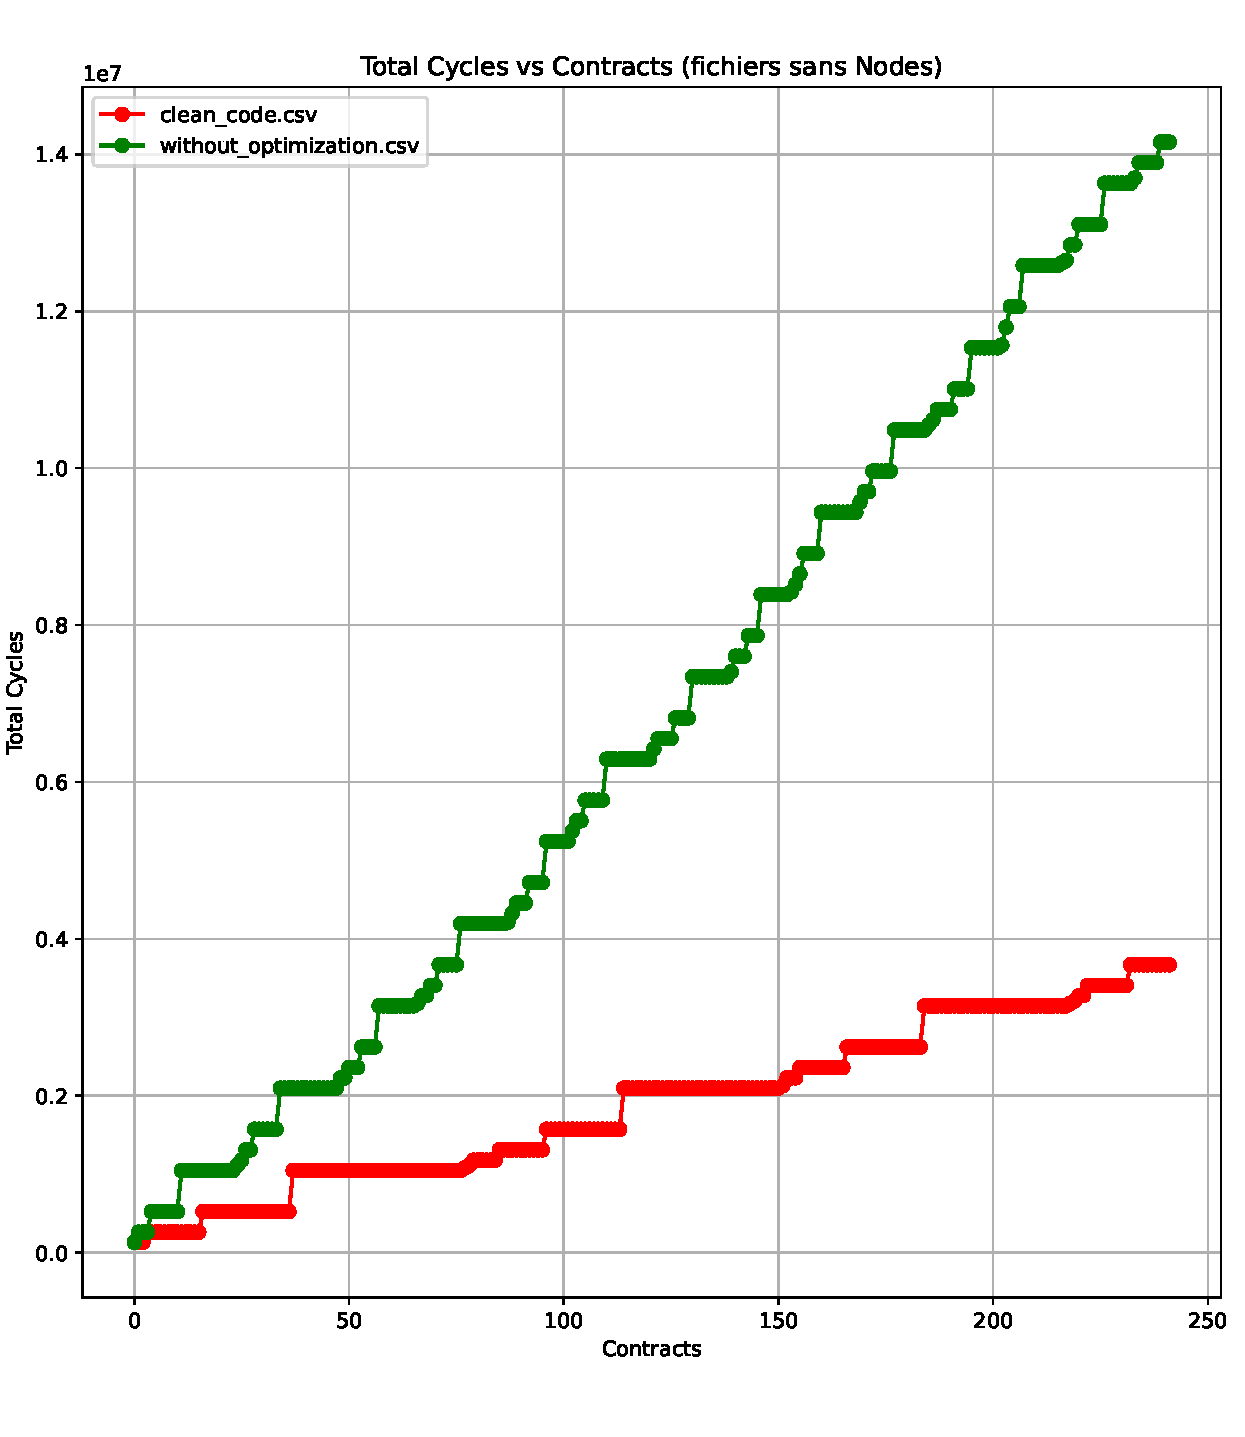
\includegraphics[width=0.4\textwidth]{benchmark_indusnet.pdf}
    \caption{Temps de calcul des bornes de latences sur un réseau industriel, 
    (on observe des pics dans
    les courbes, ce sont des arrondissements de cycles pour la génération de preuves, étant donné qu'elle travail avec des cycles ronds).}
\end{figure}



% --------- TFA++ ---------
\chapter{Ouverture sur l'algorithme TFA++}

Après l'objectif principal du stage qui était d'optimiser la génération de preuves.
J'ai pu intégrer un deuxième algorithme : TFA++.

\bigskip

\textbf{TFA++} est extension plus précise de TFA, qui 
\textbf{intègre explicitement les temps de transmission sur les 
liens entre les nœuds}. Autrement dit, l'algorithme modélise la 
progression réelle des paquets dans le réseau. Grâce à cette modélisation plus fine, 
TFA++ fournit des \textbf{bornes de délai moins pessimistes} et 
donc plus proches du comportement réel du système.

\bigskip

Ce gain en précision a toutefois un coût: en tenant compte des 
liens, le traitement est plus complexe, ce qui se traduit 
par un \textbf{temps de calcul plus long}. Mais dans les 
systèmes critiques, par exemple les réseaux embarqués dans 
l'aéronautique ou l'automobile, cette précision accrue est 
souvent indispensable pour garantir des propriétés de sûreté.

\bigskip

Ainsi, TFA++ \textbf{représente un compromis} entre rapidité 
d'analyse et fidélité du modèle, en choisissant de 
sacrifier un peu de performance pour obtenir des résultats 
significativement plus réalistes.

\break{}

\section{Méthode de calcul avec TFA++}

Avant d'implémenter ce nouvel algorithme, il faut d'abord
comprendre comment ce dernier diverge dans les calculs par
rapport à \textbf{TFA}.

\bigskip

Avec TFA, pour chaque classe de priorité, et à chaque nœud,
on récupérait l'ensemble des flux arrivant à ce dit nœud.

\smallskip

TFA fait ensuite la somme de ces flux entrants $\alpha_B$, afin d'obtenir la 
courbe d'entrée du nœud étudiée. Une fois cette courbe obtenue,
il nous suffit de récupérer la courbe de service $\beta_B$ du nœud,
c'est-à-dire la courbe représentant la capacité d'envoi du nœud.

\smallskip

Enfin, on calcule la distance horizontale maximale entre la courbe $\alpha_B$
et la courbe de service $\beta_B$, représentant le temps $D_B$ pour qu'un bit
soit envoyé par le nœud.

\bigskip

\vspace{0.5cm}

\begin{figure}[h!]
\begin{center}
\begin{tikzpicture}
    \node[anchor=south east] at (-1,0) (ina) {% !TeX spellcheck = en_US
% !TeX program = lualatex
% !TeX root = ludovic
\begin{tikzpicture}[anchor=center]
	\pgfplotsset{ticks=none}
	\begin{axis}[
		xlabel=t,
		xmin=-2,
		xmax=6,
		ymin=-1,
		ymax=7,
		axis lines=center,
		width=7cm,
		height=5cm
	]
	\tikzstyle{ma} = [
        shorten >=-3.5pt,
        shorten <=-3.5pt
    ]
	\node[anchor=north east] at (axis cs:0,6) {data};
	\addplot[{Circle[open]}-, ma, domain=0:6, color=orange, line width=1.5pt]{0.5*x+3} node[left, pos=0]{$b_{f,A'}$}  node[above, pos=0.5, sloped]{rate $r_f$} node[pos=0.9,below,sloped]{$\alpha_{f,A'}$};
	\addplot[-Circle, ma, domain=-2:0, color=orange, line width=1.5pt]{0};


	
\end{axis}
\end{tikzpicture}
};
    \node[anchor=south west] at (1,0) (inb) {% !TeX spellcheck = en_US
% !TeX program = lualatex
% !TeX root = ludovic
\begin{tikzpicture}[anchor=center]
	\pgfplotsset{ticks=none}
	\begin{axis}[
		xlabel=t,
		xmin=-2,
		xmax=6,
		ymin=-1,
		ymax=7,
		axis lines=center,
		width=7cm,
		height=5cm
	]
	\tikzstyle{ma} = [
        shorten >=-3.5pt,
        shorten <=-3.5pt
    ]
	\node[anchor=north east] at (axis cs:0,6) {data};
	\addplot[{Circle[open]}-, ma, domain=0:6, color=orange, line width=1.5pt]{0.75*x+2.5} node[left, pos=0]{$b_{h,E'}$}  node[above, pos=0.5, sloped]{rate $r_h$} node[pos=0.9,below,sloped]{$\alpha_{h,E'}$};
	\addplot[-Circle, ma, domain=-2:0, color=orange, line width=1.5pt]{0};


	
\end{axis}
\end{tikzpicture}
};
    \node[orange, rounded corners=0.5cm, fit={(ina)}, draw, line width=1.5pt] (a) {};
    \node[orange, rounded corners=0.5cm, fit={(inb)}, draw, line width=1.5pt] (b) {};
    \node at (0,-1) (sum) {\Huge ${\boldsymbol{\oplus}}$};
    \draw[-latex, line width=1.5pt, shorten >= 0.3cm] (a) -- (sum.center);
    \draw[-latex, line width=1.5pt, shorten >= 0.3cm] (b) -- (sum.center);
    \draw[-latex, line width=1.5pt, shorten <= 0.3cm] (sum.center) -- ++(0,-3);

    \node[anchor=north] at (0,-2) (compute) {% !TeX spellcheck = en_US
% !TeX program = lualatex
% !TeX root = ludovic
\begin{tikzpicture}[anchor=center]
	\pgfplotsset{ticks=none}
	\begin{axis}[
		xlabel=t,
		xmin=-2,
		xmax=6,
		ymin=-2,
		ymax=12,
		axis lines=center,
		width=14cm,
		height=8cm
	]
	\tikzstyle{ma} = [
        shorten >=-3.5pt,
        shorten <=-3.5pt
    ]
	\node[anchor=north east] at (axis cs:0,15) {data};
	\addplot[{Circle[open]}-, ma, domain=0:6, color=orange, line width=1.5pt]{0.5*x+3+0.75*x+2.5} node[left, pos=0]{$b_{f,A'}+b_{h,E'}$}  node[above, pos=0.5, sloped]{rate $r_f+r_h$} node[pos=0.7,below,sloped]{$\alpha_{f,A'}+\alpha_{h,E'}$};
	\addplot[-Circle, ma, domain=-2:0, color=orange, line width=1.5pt]{0};


    \addplot[domain=1:6, color=OliveGreen]{2*x-2} node[below, pos=0]{$T_B$} node[below,pos=0.6,sloped]{rate $R_B$} node[pos=0.9,above,sloped] {$\beta_{B}$};
	\addplot[domain=-2:1, color=OliveGreen]{0};

	\draw[latex-latex, red] (axis cs:0,5.5) -- (axis cs:3.75,5.5) node[pos=0.5, above] {\makecell{$D_B$}};


	
\end{axis}
\end{tikzpicture}
};
\end{tikzpicture}
\end{center}
\caption{Schéma synthétisant le comportement de TFA}
\end{figure}

\break{}

Pour TFA++, nous ne faisons plus la somme des courbes des flux entrants,
mais on construit la courbe minimale de ces courbes. La courbe de 
service du nœud est calculée de la même manière, et la recherche
de la distance maximale entre la courbe d'entrée et la courbe de
service est obtenue en récupérant le maximum des différents 
distances horizontales entre les points de changement de pente
et la courbe de service.

\bigskip

\vspace{0.5cm}
\begin{figure}[h!]
\begin{center}
\begin{tikzpicture}
    \node[anchor=south east] at (-1,0) (ina) {% !TeX spellcheck = en_US
% !TeX program = lualatex
% !TeX root = ludovic
\begin{tikzpicture}[anchor=center]
	\pgfplotsset{ticks=none}
	\begin{axis}[
		xlabel=t,
		xmin=-2,
		xmax=6,
		ymin=-1,
		ymax=7,
		axis lines=center,
		width=7cm,
		height=5cm
	]
	\tikzstyle{ma} = [
        shorten >=-3.5pt,
        shorten <=-3.5pt
    ]
	\node[anchor=north east] at (axis cs:0,6) {data};
	\addplot[{Circle[open]}-, shorten <=-3.5pt, domain=0:0.5714285714285714, color=orange, line width=1.5pt, dotted]{0.5*x+3} node[left, pos=0]{$b_{f,A'}$};
    \addplot[domain=0.5714285714285714:6, color=orange, line width=1.5pt]{0.5*x+3}  node[above, pos=0.5, sloped]{rate $r_f$} node[pos=0.9,below,sloped]{$\alpha_{f,A'}$};
	\addplot[-Circle, ma, domain=-2:0, color=orange, line width=1.5pt]{0};

    \addplot[{Circle[open]}-, shorten <=-3.5pt, domain=0:0.5714285714285714, color=black, line width=1.5pt]{4*x+1} node[left, pos=0]{$L^{\max}_{(A,B)}$} ;
    \addplot[domain=0.5714285714285714:6, color=black, line width=1.5pt, dotted]{4*x+1} node[above, pos=0.1, sloped]{rate $c_A$};
	\addplot[-Circle, ma, domain=-2:0, color=black, line width=1.5pt]{0};


	
\end{axis}
\end{tikzpicture}
};
    \node[anchor=south west] at (1,0) (inb) {% !TeX spellcheck = en_US
% !TeX program = lualatex
% !TeX root = ludovic
\begin{tikzpicture}[anchor=center]
	\pgfplotsset{ticks=none}
	\begin{axis}[
		xlabel=t,
		xmin=-2,
		xmax=6,
		ymin=-1,
		ymax=7,
		axis lines=center,
		width=7cm,
		height=5cm
	]
	\tikzstyle{ma} = [
        shorten >=-3.5pt,
        shorten <=-3.5pt
    ]
	\node[anchor=north east] at (axis cs:0,6) {data};
	\addplot[{Circle[open]}-, shorten <=-3.5pt, domain=0:0.46153846153846156, color=orange, line width=1.5pt, dotted]{0.75*x+2.5} node[left, pos=0]{$b_{h,E'}$};
    \addplot[domain=0.46153846153846156:6, color=orange, line width=1.5pt]{0.75*x+2.5}  node[above, pos=0.5, sloped]{rate $r_h$} node[pos=0.85,below,sloped]{$\alpha_{h,E'}$};
	\addplot[-Circle, ma, domain=-2:0, color=orange, line width=1.5pt]{0};

    \addplot[{Circle[open]}-, shorten <=-3.5pt, domain=0:0.46153846153846156, color=black, line width=1.5pt]{4*x+1} node[left, pos=0]{$L^{\max}_{(E,B)}$} ;
    \addplot[domain=0.46153846153846156:6, color=black, line width=1.5pt, dotted]{4*x+1} node[above, pos=0.1, sloped]{rate $c_E$};
	\addplot[-Circle, ma, domain=-2:0, color=black, line width=1.5pt]{0};


	
\end{axis}
\end{tikzpicture}
};
    \node[orange, rounded corners=0.5cm, fit={(ina)}, draw, line width=1.5pt] (a) {};
    \node[orange, rounded corners=0.5cm, fit={(inb)}, draw, line width=1.5pt] (b) {};
    \node at (0,-1) (sum) {\Huge ${\boldsymbol{\oplus}}$};
    \draw[-latex, line width=1.5pt, shorten >= 0.3cm] (a) -- (sum.center);
    \draw[-latex, line width=1.5pt, shorten >= 0.3cm] (b) -- (sum.center);
    \draw[-latex, line width=1.5pt, shorten <= 0.3cm] (sum.center) -- ++(0,-3);

    \node[anchor=north] at (0,-2) (compute) {% !TeX spellcheck = en_US
% !TeX program = lualatex
% !TeX root = ludovic
\begin{tikzpicture}[anchor=center]
	\pgfplotsset{ticks=none}
	\begin{axis}[
		xlabel=t,
		xmin=-2,
		xmax=6,
		ymin=-2,
		ymax=12,
		axis lines=center,
		width=14cm,
		height=8cm
	]
	\tikzstyle{ma} = [
        shorten >=-3.5pt,
        shorten <=-3.5pt
    ]
	\node[anchor=north east] at (axis cs:0,15) {data};
	\addplot[{Circle[open]}-, ma, domain=0:0.5714285714285714, color=orange, line width=1.5pt, dotted]{0.5*x+3+0.75*x+2.5} node[left, pos=0]{$b_{f,A'}+b_{h,E'}$};
    \addplot[domain=0.5714285714285714:6, color=orange, line width=1.5pt]{0.5*x+3+0.75*x+2.5}node[above, pos=0.5, sloped]{$r_f+r_h$} node[pos=0.7,below,sloped]{$\alpha_{f,A'}+\alpha_{h,E'}$};


    \addplot[domain=1:6, color=OliveGreen]{2*x-2} node[below, pos=0]{$T_B$} node[below,pos=0.6,sloped]{rate $R_B$} node[pos=0.9,above,sloped] {$\beta_{B}$};
	\addplot[domain=-2:1, color=OliveGreen]{0};

	\draw[latex-latex, red] (axis cs:0,2) -- (axis cs:2,2) node[pos=0.5, above] {\makecell{$D^1$}};
    \draw[latex-latex, red] (axis cs:0.46153846153846156,5.6923076923076925) -- (axis cs:3.8461538461538463,5.6923076923076925) node[pos=0.5, below] {\makecell{$D^2$}};

    \draw[latex-latex, red] (axis cs:0.5714285714285714,6.2142857142857135) -- (axis cs:4.107142857142857,6.2142857142857135) node[pos=0.5, above] {\makecell{$D^3$}};
    
    


    \addplot[{Circle[open]}-, shorten <=-3.5pt, domain=0:0.46153846153846156, color=orange, line width=1.5pt]{8*x+2} node[left, pos=0]{$L^{\max}_{(A,B)}+L^{\max}_{(E,B)}$} ;
    \addplot[domain=0.46153846153846156:6, color=orange, line width=1.5pt, dotted]{8*x+2} node[above, pos=0.1, sloped]{$c_E+c_A$};
	\addplot[-Circle, ma, domain=-2:0, color=orange, line width=1.5pt]{0};

    \addplot[domain=0.46153846153846156:0.5714285714285714, color=orange, line width=1.5pt]{4*x+1+0.75*x+2.5};
    \addplot[domain=0.5714285714285714:6, color=orange, line width=1.5pt, dotted]{4*x+1+0.75*x+2.5} node[above, pos=0.15, sloped]{$c_E$};


	
\end{axis}
\end{tikzpicture}
};
\end{tikzpicture}
\end{center}
\caption{Schéma synthétisant le comportement de TFA++}
\end{figure}

\break{}

\section{Implémentation de TFA ++}

Dans cette partie, nous allons voir les différentes structures
et méthodes qui ont été ajouté et adapté dans le code initiale
de TFA pour transitionner sur le comportement de TFA++.

\subsection*{1. Structures de base}

\subsubsection*{Segment}

Chaque segment représente une droite de la forme :
\[
\alpha(t) = b + r \cdot t
\]
où $b$ est le \textit{burst} et $r$ le \textit{rate}.

\subsubsection*{Curve}

Une courbe est une suite ordonnée de segments.
Chaque segment est ajouté avec soin pour garantir que la courbe 
reste minimale.

\subsection*{2. Méthodes principales}

\subsubsection*{add\_segment}

Cette méthode \textbf{ajoute un segment} à la courbe existante en vérifiant plusieurs propriétés :

\begin{itemize}
  \item Supprimer les segments dominants.
  \item Maintenir l'ordre croissant des points d'intersection.
\end{itemize}

\subsubsection*{sum\_curve}

Permet de \textbf{combiner deux courbes}. Pour chaque paire de segments $(s_1, s_2)$, on génère un nouveau segment $s$ tel que :
\[
s.\text{rate} = s_1.\text{rate} + s_2.\text{rate}, \quad
s.\text{burst} = s_1.\text{burst} + s_2.\text{burst}
\]

La courbe résultante est ensuite minimisée par \texttt{add\_segment}.

\subsubsection*{get\_intersection\_points}

Cette méthode retourne les points d'intersection entre segments successifs :
\[
x = \frac{b_2 - b_1}{r_1 - r_2}, \quad
y = r_1 \cdot x + b_1
\]

Ces points sont utiles pour déterminer les ponts de changement
de pente dans la courbe, nécessaires pour le calcul de la borne de délai.

\subsubsection*{compute\_class\_delay\_bound}

Calcule la borne de délai maximale selon le service d'un nœud $n$:
\[
D_n = T_n + \frac{\alpha_n(t)}{R_n} - t
\]
où :
\begin{itemize}
  \item $D_n$ est le délai maximum subit par un bit entrant,
  \item $T_n$ est la latence de service,
  \item $R_n$ le débit de service,
  \item $\alpha_n(t)$ est la courbe d'entrée.
  \item $t$ désigne les moments correspondant aux changements de pente.
\end{itemize}


\section{Performances de TFA++}




% --------- Conclusion ---------
\chapter{Conclusion}
[Bilan, récapitulatif des apports, ouverture.]

[TODO : Citer ludovic sur les captions
        Travaille réalisé avec Mathieu AMET sur les captions du code
        Faire Bibliographie
        Et citer le boss docquier]

% --------- Bibliographie ---------
%\printbibliography


\end{document}
